% !TEX TS-program = pdflatex
% !TEX encoding = UTF-8 Unicode

% This is a simple template for a LaTeX document using the "article" class.
% See "book", "report", "letter" for other types of document.

%tells you if you use obsolote packages
%\RequirePackage[l2tabu,orthodox]{nag}

\documentclass[]{article}

\usepackage[utf8]{inputenc} % set input encoding (not needed with XeLaTeX)

%%% PAGE DIMENSIONS
\usepackage{geometry} % to change the page dimensions
\geometry{a4paper} % or letterpaper (US) or a5paper or....
% \geometry{margin=2in} % for example, change the margins to 2 inches all round
% \geometry{landscape} % set up the page for landscape
%   read geometry.pdf for detailed page layout information

\usepackage{graphicx} % support the \includegraphics command and options

% \usepackage[parfill]{parskip} % Activate to begin paragraphs with an empty line rather than an indent

%%% PACKAGES
\usepackage{booktabs} % for much better looking tables
\usepackage{array} % for better arrays (eg matrices) in maths
\usepackage{paralist} % very flexible & customisable lists (eg. enumerate/itemize, etc.)
\usepackage{verbatim} % adds environment for commenting out blocks of text & for better verbatim
\usepackage{subfig} % make it possible to include more than one captioned figure/table in a single float
\usepackage{microtype} %makes awesome kerning and punctuation come half way out the edge of the text
\usepackage{listings} %for code listings
\usepackage{color} %for colored syntax highligting
\usepackage{rotating}
\usepackage{pdflscape}

%%% Code listing
\definecolor{mygreen}{rgb}{0,0.6,0}
\definecolor{mygray}{rgb}{0.5,0.5,0.5}
\definecolor{mymauve}{rgb}{0.58,0,0.82}
\lstset{breaklines=true,
basicstyle=\footnotesize\ttfamily,
commentstyle=\color{mygreen},
keywordstyle=\color{blue},
numberstyle=\tiny\color{mygray},
tabsize=2,
frame=tb,
aboveskip=5mm,
belowskip=0mm,
breaklines=true,
breakatwhitespace=true
}

% to include a file as a listing: \lstinputlisting{intio.c}
% inline listing: \begin{lstlisting}[frame=single]

%%% HEADERS & FOOTERS
\usepackage{fancyhdr} % This should be set AFTER setting up the page geometry
\pagestyle{fancy} % options: empty , plain , fancy
\renewcommand{\headrulewidth}{0pt} % customise the layout...
\lhead{}\chead{}\rhead{}
\lfoot{}\cfoot{\thepage}\rfoot{}

%%% ToC (table of contents) APPEARANCE
\usepackage[nottoc,notlof,notlot]{tocbibind} % Put the bibliography in the ToC
\usepackage[titles,subfigure]{tocloft} % Alter the style of the Table of Contents
%\renewcommand{\cftsecfont}{\rmfamily\mdseries\upshape}
%\renewcommand{\cftsecpagefont}{\rmfamily\mdseries\upshape} % No bold!
\usepackage{hyperref} % use hyperlinked ToC
\hypersetup{colorlinks=true, linkcolor=black}

%%%-------------------------------------------------------------------


\title{Digital System Design Report}
\author{Oskar Weigl - ow610\\ and \\ Ryan Savitski - rs510}
%\date{} % Activate to display a given date or no date (if empty),
         % otherwise the current date is printed 

\begin{document}
\maketitle

%\renewcommand{\abstractname}{Summary}
\begin{abstract}
	Write the abstract here
\end{abstract}

\tableofcontents
\clearpage

\section{Floating Point Hardware} % (fold)
\label{sec:floating_point_hardware}

% section floating_point_hardware (end)

\section{Determinant Calculation Hardware Accelerator} % (fold)
\label{sec:determinant_calculation_hardware_accelerator}

\begin{table}[htbp]
	\caption{Resource Utilisation of the Determinant module. Note that two fp\_mul units are used.}
	\label{tab:resource_util_det}
	\begin{center}
		\begin{tabular}{l|ccccc}
		\hline

		\hline
											& \textbf{Entire Module} 	& \textbf{fp\_div} 		& \textbf{fp\_mul}	& \textbf{fp\_sub} 	& \textbf{matrixram} \\
		\hline
			\textbf{Logic Cells} 			& 5978						& 404 					& 264 				& 827 				& 0 \\
		\hline
			\textbf{Dedicated Registers}	& 3663						& 291 					& 208 				& 426				& 0 \\
		\hline
			\textbf{M9K Memory Blocks}		& 11						& 6 					& 0 				& 1 				& 4 \\
		\hline
			\textbf{Multiplier Elements}	& 31						& 16 					& 7 				& 0					& 0 \\
		\hline

		\hline
		\end{tabular}
	\end{center}
\end{table}

\begin{figure}[htbp]
	\begin{center}
		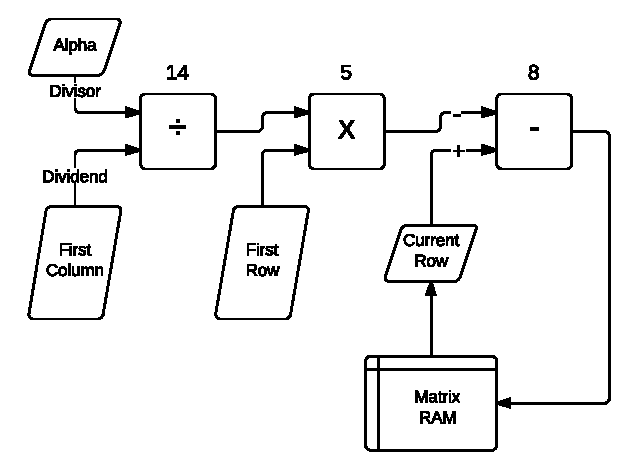
\includegraphics[width = 0.8\textwidth]{DeterminantPipeline.pdf}
	\end{center}
	\caption{Block diagram of the hardware implementation of the Doolittle Algorithm.}
	\label{fig:det_block}
\end{figure}





% section determinant_calculation_hardware_accelerator (end)


\clearpage


\section{Notch Filter} % (fold)
\label{sec:notch_filter}

The Notch Filter module is a memory mapped hardware accelerator for the purpose of filtering a 16 bit signed input. It is a 2nd order notch filter tuned to to remove any spectral components at 1 kHz.
The module is capable of Direct Memory Access, and includes optimisations for efficient access to the SDRAM, and uses a buffering, and Clock Domain Crossing strategy, to maximise performance.

\subsection{Filter Design} % (fold)
\label{sub:filter_design}

Several different types of filter topologies are considered. Firstly, it is clear that as a 2nd order IIR filter meets the specification, it would be rather inappropriate to implement the same filter as an FIR filter. To get the same sharp transition band using an FIR filter, we would have to use over 10,000 taps. This metric is generated using MATLAB's Parks-McClellan optimal equiripple FIR order estimator; the MATLAB command and result can be seen in Figure~\ref{fig:firpmord}.

\begin{figure}[htbp]
	\begin{center}
		\begin{lstlisting}[language = Matlab]
beethmax = max(abs(fft(beeth5_noise)));
firpmord([987.5 999 1001 1012.5], [1 0 1], [0.01 10/beethmax 0.01], 44100)
ans = 13410
		\end{lstlisting}
	\end{center}
	\caption{MATLAB command to estimate the order of FIR filter required for the notch filter specification.}
	\label{fig:firpmord}
\end{figure}

The chosen filter type is a 2nd order IIR filter. This filter order is the minimum required to generate the complex pole and zero pairs required to implement a notch filter. In fact, no higher order is needed, as the noise is a pure sinusoid, so the width of the stop-band can be very small, and as such, there are no additional zeroes required.

The filter is designed by simply placing a complex zero pair on the unit circle corresponding to the 1 KHz null we wish to create. To cancel the effect of this zero for other frequencies, we place a pole very close to it on the inside of the unit circle. The bandwidth of the filter is tuned by moving the complex pole radially.

In our case, we elect to place the pole such that the bandwidth of rejection is about 25Hz. This is is chosen as a good trade-off for several reasons. Firstly, placing the pole at this location makes the filter robust to coefficient quantisation, as discussed in Section~\ref{sub:quantization}.
More importantly, this bandwidth is narrow enough to not affect the music, but wide enough to quickly suppress the overlaid sinusoid at the beginning of the sample.
The magnitude of the resulting filter can been seen in Figure~\ref{fig:matlabmagnitudelog}.

\begin{figure}[htbp]
	\begin{center}
		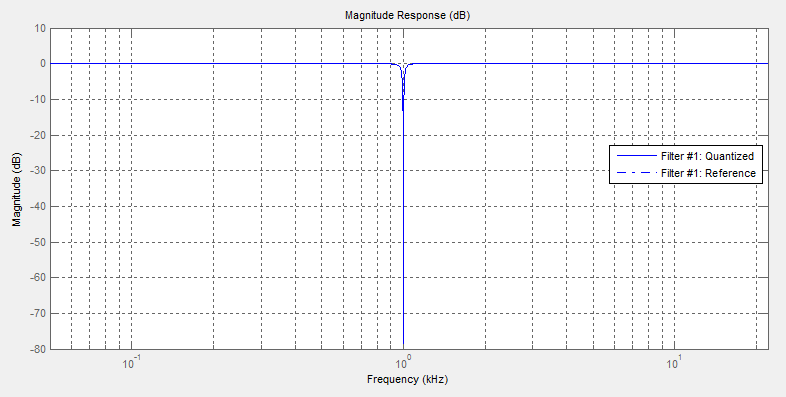
\includegraphics[width = \textwidth]{matlabmagnitudelog.PNG}
	\end{center}
	\caption{Magnitude response of both the full (double) precision and the quantised filter. The gain is negative infinity dB at 1 kHz.}
	\label{fig:matlabmagnitudelog}
\end{figure}

% subsection filter_design (end)

\subsection{Filter Topology} % (fold)
\label{sub:filter_topology}

\begin{figure}[btp]
	\begin{center}
		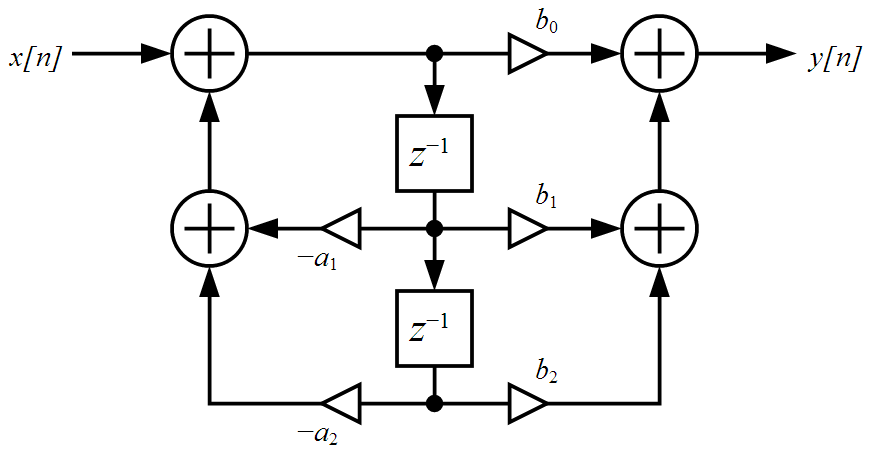
\includegraphics[width = 0.75\textwidth]{dfII.PNG}
	\end{center}
	\caption{Second order Direct Form II filter topology.}
	\label{fig:dfII}
\end{figure}

\begin{figure}[tbp]
	\begin{center}
		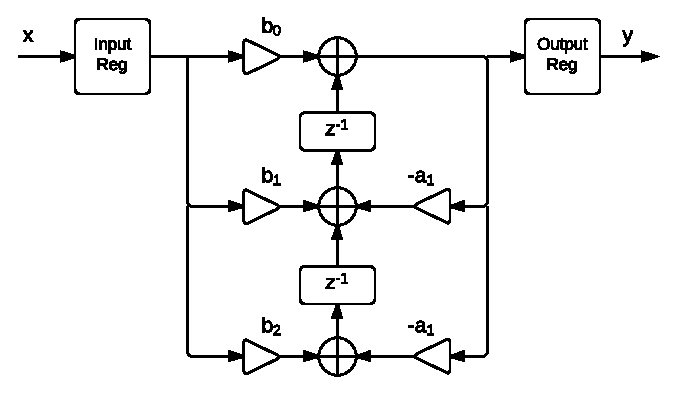
\includegraphics[width = 0.9\textwidth]{DirectFormIITransposed.pdf}
	\end{center}
	\caption{Second order Direct Form II Transposed filter topology.}
	\label{fig:df2t}
\end{figure}

As a second order IIR filter is settled upon, we need to chose what filter topology we will use. The candidates are Direct Forms I and II, and their transposed versions. It is immediately clear that the Direct Form II versions are better than the Direct Form I, as the number of state registers can be halved. Thus, the choice remains between regular and transposed version of Direct Form II.

In a software implementation, the difference between the two would be quite small, but in a hardware implementation they differ significantly. As can be seen in Figure~\ref{fig:dfII}, the Direct Form II filter topology requires an adder chain on the feedback path. This adder chain adds one adder in a chain for every added order of the filter.

Conversely, the Direct Form II Transposed filter topology only has a single 3-input adder for each stage, which is invariant to the filter order, as illustrated by Figure~\ref{fig:df2t}.
Thus, for the critical path is constant for any order of the filter, and in all cases shorter than the non-transposed version. The timing of the filter is explored further in Section~\ref{sub:timing_analysis}.

% subsection filter_topology (end)

\begin{table}[htb]
	\begin{center}
		\begin{lstlisting}
   FilterStructure: 'Direct-Form II Transposed, Second-Order Sections'
        Arithmetic: 'fixed'
         Numerator: [1 -1.979736328125 1]                  
       Denominator: [1 -1.97576904296875 0.996002197265625]
  PersistentMemory: false

   CoeffWordLength: 18                
     NumFracLength: 16                
     DenFracLength: 16
            Signed: true              
                                      
   InputWordLength: 16                
   InputFracLength: 0                 
                                      
  OutputWordLength: 16
  OutputFracLength: 0                 
                                      
   StateWordLength: 18
   StateFracLength: 2                 
                                      
 ProductWordLength: 36                
 NumProdFracLength: 16                
 DenProdFracLength: 16                
                                      
   AccumWordLength: 18                
NumAccumFracLength: 1                 
DenAccumFracLength: 1                 

         RoundMode: 'convergent'      
      OverflowMode: 'wrap'  
		\end{lstlisting}
	\end{center}
	\caption{Fixed point filter designed in MATLAB.}
	\label{tab:Hdsdsos}
\end{table}

\subsection{Quantization} % (fold)
\label{sub:quantization}

The effects of quantization depends entirely on the chosen filter topology. An FIR filter, which has no poles (except at the origin), can never go unstable, and as such, it is less sensitive to coefficient quantization. However, as seen in Section~\ref{sub:filter_design}, an FIR filter is simply not feasible for this application. Thus, as an IIR filter is required, careful consideration of the effects of quantization is required.

As this is a hardware implementation, it is possible to independently designate the bit widths for each of the different stages of the filter. That is, it is not only the bit width of the coefficients themselves that need to be tuned, but also the width of the data-paths, the input, the output, the state registers, the multipliers, and the adders. Furthermore, the resources of the target hardware architecture has to be considered.
For instance, the target FPGA has hardware multipliers that either multiply two 9 bit numbers, or alternatively, multiply two 18 bit numbers. That is, any bit-width between these two values would be underutilising the resources available on the FPGA.

During the initial design of the filter, it was established that a minimum of 12 bits was required for the coefficients of the filter in order to not create any resonance in the filter which would artificially amplify a portion of the passband.
Furthermore, it was empirically found that playback of the audio at 8 bits was simply not high enough fidelity to do the music justice. At 16 bits, the audio was deemed to be of good enough quality, and as such, the input and output widths of the filter are chosen to be 16 bits.

As we require at least 12 bits wide coefficients, and as the multipliers will have to be 18 bits wide, it is no penalty in terms of hardware resources to simply elect to have 18 bits wide coefficients. That is, as the coefficients do not have to change during runtime, no registers are required to hold the coefficients.
Furthermore, as the coefficients are 18 bits, and the input is 16 bits, the rest of the system is required to be at least 16 bits wide in order to preserve the precision. However, as the adder and state stages are in series, it is in fact beneficial to have 2-3 more bits. Thus, it is elected to set the adder and state register bit-widths to 18 bits.

Finally, we must consider where to place the binary point in the fixed point representation. As this is a hardware implementation, shifts of the binary point are free. In order to scale the binary point, we used the command \verb"Hdsdsos = autoscale(Hdsdsos, x)" from the digital filter toolbox in MATLAB.
This command will automatically scale the binary point of the different stages of the filter. It uses the provided input (in this case a 16 bit signed integer sample of the noisy music) to scale the binary point to include as much precision as possible while still avoiding overflow. The result of the operation can be seen in Figures~\ref{tab:Hdsdsos} and \ref{tab:fixedpoint_report}.

\begin{table}[htbp]
	\begin{center}
		\begin{lstlisting}
                               Fixed-Point Report                                          
            -------------------------------------------------------------------
                  Min       Max     |        Range       | Number of Overflows
            -------------------------------------------------------------------
      Input:      -32768      32767 |   -32768     32767 |   0/963144 (0%)
 Section In:      -32768      32767 |   -32768     32767 |  0/1926288 (0%)
Section Out:      -23436      23293 |  -131072    131071 |  0/1926288 (0%)
     Output:      -23436      23293 |   -32768     32767 |   0/963144 (0%)
     States:      -16423    16408.5 |   -32768  32767.75 |  0/1926288 (0%)
   Num Prod:   -64870.02      64872 |  -524288    524288 |  0/2889432 (0%)
   Den Prod:  -46021.588  46304.123 |  -524288    524288 |  0/1926288 (0%)
    Num Acc:      -64870      64872 |   -65536   65535.5 |  0/1926288 (0%)
    Den Acc:    -54472.5      54347 |   -65536   65535.5 |  0/1926288 (0%)
		\end{lstlisting}
	\end{center}
	\caption{Filtering Report generated when filtering the input sample}
	\label{tab:fixedpoint_report}
\end{table}

% subsection quantization (end)


\subsection{Filter Implementation} % (fold)
\label{sub:filter_implementation}

The filter described in Section~\ref{sub:quantization} is engineered to minimise quantisation noise while avoiding any overflow. This design is carried out using the digital filter toolbox in MATLAB.
This toolbox includes a feature for outputting the custom filter design as automatically generated Hardware Description Language (HDL).
Using the \verb"fdhdltool" command, we are able to generate Verilog HDL from the filter we have designed.

As this method is guaranteed to generate the same digital filter that is already extensively tested in MATLAB, we are able to save a great deal of time in design and especially debugging of the filter core itself.
The time saved is put to use in performing the integration of the filter with the rest of the system, and especially in developing the custom memory controller described in Section~\ref{sub:hardware_implementation} and \ref{sub:tuning_for_speed}.

This tool provides us with a Verilog source file with the interface as shown in Figure~\ref{fig:Hdsdsos_interface}. The filter input and outputs are signed 16 bit integer representation with no fractional parts, as required.

The HDL generation tool can also generate a second type of interface, one specifically designed to be capable of interfacing to a CPU for loading custom coefficients. However, due to the optimisations described in Section~\ref{sub:timing_analysis}, we elected to use hard-wired coefficients.
That is, the filter design tool cannot assume that the overall gain of the filter is unity when electing to supply coefficients from the processor interface.

However, it is possible to modify four (and with some modifications, five) out of the six coefficients while still maintaining the speed advantage. This design alteration is described in Section~\ref{sub:timing_analysis}, but we did not have time to implement it.
As such, while it would be possible to have a fast system with variable coefficients, the system as it stands, has hard-wired coefficients.

\begin{figure}[bt]
	\begin{center}
		\begin{lstlisting}[language = Verilog]
module Hdsdsos_copy_hardwired
               (
                clk,
                clk_enable,
                reset,
                filter_in,
                filter_out
                );

input   clk; 
input   clk_enable; 
input   reset; 
input   signed [15:0] filter_in; //sfix16
output  signed [15:0] filter_out; //sfix16
		\end{lstlisting}
	\end{center}
	\caption{The interface of the automatically generated filter.}
	\label{fig:Hdsdsos_interface}
\end{figure}

% subsection filter_implementation (end)

\subsection{Hardware Implementation} % (fold)
\label{sub:hardware_implementation}

% \begin{figure}[htbp]
% 	\begin{center}
% 		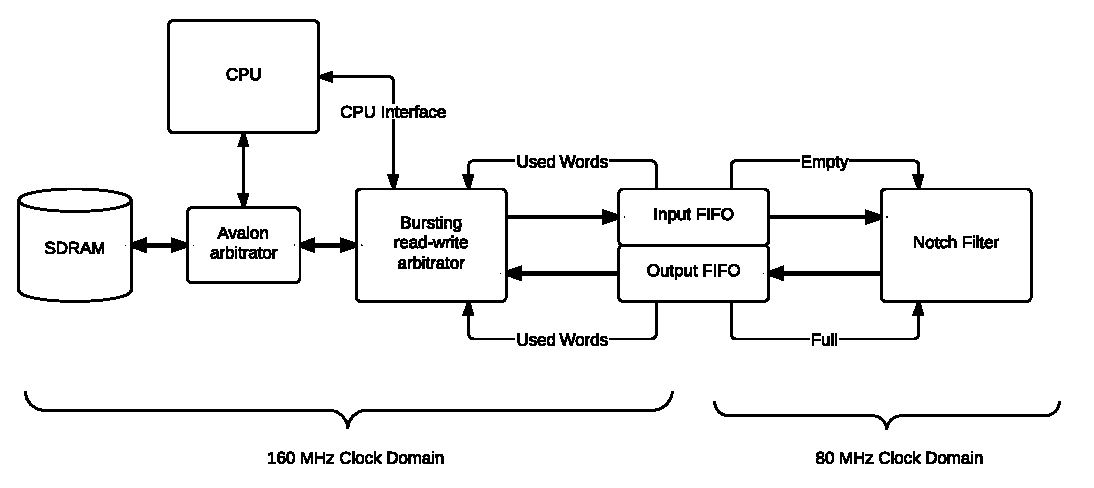
\includegraphics[width = \textwidth]{DSDNotch.pdf}
% 	\end{center}
% 	\caption{Block diagram of the Notch Filter hardware. FIFO buffers are used to allow efficient interleaved reads and writes to SDRAM. The buffers also serve as Clock Domain Crossing interfaces.}
% 	\label{fig:DSDNotch}
% \end{figure}



The filtering module, depicted in Figure~\ref{fig:DSDNotch}, is implemented as a memory mapped device. The CPU communicates with the hardware block by writing to a Avalon slave interface.
The hardware module also has a Avalon Memory-Mapped Master interface so that the data required for the filtering operation can be fetched independently of the CPU, an operation known as Direct Memory Access (DMA).

The target architecture, the DE0 board, only has a single off chip memory with high memory bandwidth, the SDRAM memory. The Flash memory that is present on this board has such low memory bandwidth that if it were to be used, it would slow the system down several times over.
Thus, to complete the filtering operation, the data must be fetched from SDRAM, filtered, and then stored back in the same memory (but at a different location). The solution to this contention is to use a custom arbitrator that will interleave the reads and writes to SDRAM.

As non-sequential access to SDRAM is slow and sequential access is fast, we use a feature of the Avalon interface known as Bursting. This feature locks the slave device, in this case the SDRAM controller, and forces it to fetch or store a sequential chunk of data as one uninterrupted operation.
That is, we are able to lock the arbitration of the Avalon interconnect to finish serving our sequential burst before it interleaves any requests from other masters, such as the CPU.

In order to maximise efficiency, we use a pair of First In First Out (FIFO) buffers to absorb the data that is obtained during a read burst, or to ensure sustained write throughput during write burst.
These buffers are constructed from the architecture specific double ported memory blocks (M9K memory blocks), as shown in Figure~\ref{fig:fifoblock}.
These FIFO blocks support different clocks on the read and write ports. Thus they can be, and are, used as Clock Domain Crossing (CDC) logic. This means that we can operate the filter core at a different clock speed than the rest of the system.

The core of the filter is limited to operating at 80MHz, while the rest of the system operates at 160MHz (see Section~\ref{sub:timing_analysis} for a detailed timing analysis). This means that even though the memory access is interleaved and cannot fetch one new word every clock cycle on average, the filter can still operate at almost full saturation.

\begin{figure}[htbp]
	\begin{center}
		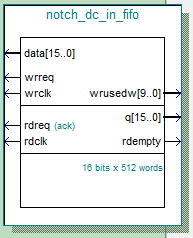
\includegraphics[width = 0.3\textwidth]{fifoBlock.PNG}
	\end{center}
	\caption{Block diagram of the First In First Out buffers used for both data buffering and Clock Domain Crossing.}
	\label{fig:fifoblock}
\end{figure}

\begin{landscape}
\begin{figure}[p]
	\begin{center}
		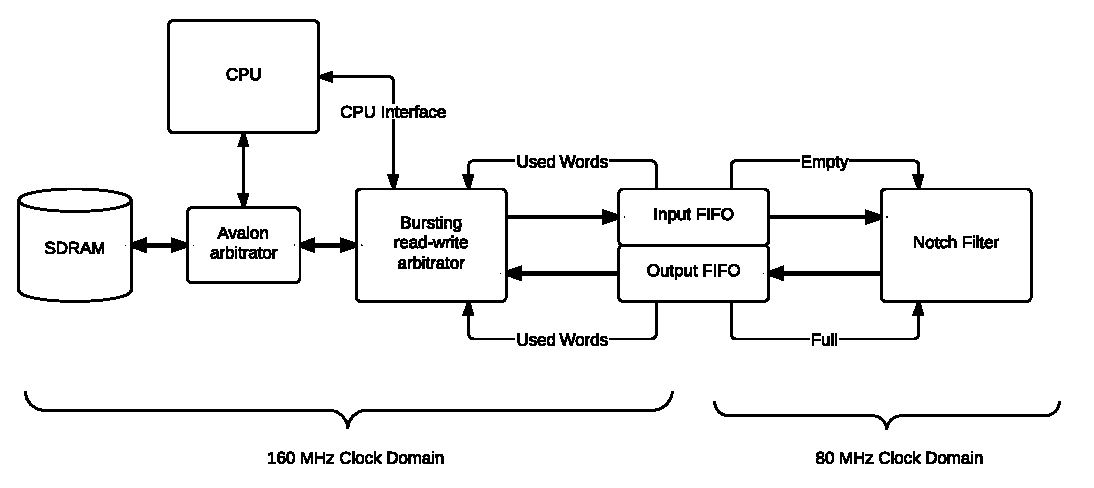
\includegraphics[width = 1.45\textwidth]{DSDNotch.pdf}
	\end{center}
	\caption{Block diagram of the Notch Filter hardware. FIFO buffers are used to allow efficient interleaved reads and writes to SDRAM. The buffers also serve as Clock Domain Crossing interfaces.}
	\label{fig:DSDNotch}
\end{figure}
\end{landscape}


% subsection hardware_implementation (end)


\subsection{Timing analysis} % (fold)
\label{sub:timing_analysis}

\begin{figure}[tbp]
	\begin{center}
		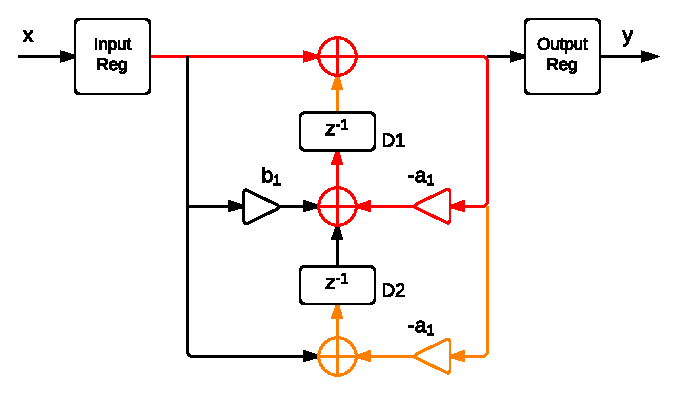
\includegraphics[width = 0.8\textwidth]{DirectFormIITransposedCritpath.pdf}
	\end{center}
	\caption{Annotated version of Figure~\ref{fig:df2t}, showing the main critical paths in the filter core. Shown in red is the critical path; from the input register to the delay register D1. Shown in orange are the alternative paths that have almost as little slack as the red path.}
	\label{fig:df2tCritpath}
\end{figure}

As mentioned in Section~\ref{sub:filter_topology}, Direct Form II Transposed is the chosen filter topology because of its superior timing characteristics. Nevertheless, the performance of the filter core is limited to processing 80 Million samples per second.
This is because the critical path, depicted in red in Figure~\ref{fig:df2tCritpath}, is forced to pass through two adder stages and one multiplier block.
Because the filter is recursive in nature, it is not possible to pipeline this path and as such it is not possible to increase the clock speed in a simple way. There is a method called Look-Ahead pipe-lining, which involves creating pole an zero pairs that cancel each other out, in order to be able to pipeline the feedback path.
However, this approach is deemed too involved for the purposes of this project.

One optimisation is however possible. As seen in Figure~\ref{fig:df2tCritpath}, the $b_0$ coefficient multiplier is not present. That is because, in our case, this coefficient, representing the overall gain of the system, is unity.
However, because of the linearity of IIR filters, if this gain is required to be non-unity, it can be moved to the other side of the input register.
Thus, the critical path is still maintained to be two adders and one multiplier for any Direct Form II Transposed filter implementation.
In our case, however, to optimise the resources used for the filter, we elected to optimise away both multiplier $b_0$ and $b_2$, as they are both unity.

Furthermore, when performing the timing analysis, we found that there are several paths that had a timing slack that is almost as tight as the critical path. These are depicted in orange in Figure~\ref{fig:df2tCritpath}.
That is, the paths from the input register to $D1$, from $D1$ to $D1$, from the input register to $D2$ and from $D1$ to $D2$, all have similar timing characteristics, and are the limiting paths in the design.

In fact, it is interesting to note that the similarity of the timing of these paths is expected expected when inspecting the data-paths in a Direct Form II Transposed filter topology. That is, as seen in Figure~\ref{fig:df2tCritpath}, all of these paths pass through two adders and one multiplier.
It is fascinating to see that the expected timing from a high level topology perspective translates so well to the final hardware implementation.

Moreover, as the FIFO buffers are used as Clock Domain Crossing interfaces, there is a risk of metastability. However as the generated clocks phase locked, as they are generated using the same PLL module, this risk is minimal.
That is, as the clock frequency ratio is an exact integer, in this case two, the clock edges should always line up, and no metastability should be possible.
Nevertheless, the FIFO buffers are set-up to use two stage synchroniser stages to synchronise operation. While this may be overkill for the purposes of eliminating metastability, it does allow register re-timing to have more freedom to optimise the circuit.  

\begin{table}[tbp]
	\caption{Timing performance of the system at various operating conditions.}
	\label{tab:fmax}
	\begin{center}
		\begin{tabular}{l|cc}
		\hline

		\hline
			 										& $0^\circ$C 					& $85^\circ$C 	\\
		\hline
			\textbf{Maximum System Frequency} 		& 181.82 MHz					& 162.0 MHz 	\\
		\hline
			\textbf{Maximum Filter Core Frequency}	& 90.59 MHz						& 80.55 MHz 	\\
		\hline
			\textbf{Metastability MTBF}				& \textgreater 1 Billion Years	& \textgreater 1 Billion Years \\
		\hline

		\hline
		\end{tabular}
	\end{center}
\end{table}

% subsection timing_analysis (end)


\subsection{Tuning for Speed} % (fold)
\label{sub:tuning_for_speed}

As the target speed of the filtering module is quite high: 160MHz for the interface side, and 80MHz for the filtering side, some special considerations are required.
In particular, it was found that the address calculation for the fetch stage of the custom memory controller could not initially operate at 160MHz.
This was because, initially, it was designed to update the current fetch pointer, compare it with the final pointer, and conditionally request new data. As these pointers are 32 bits wide, the critical path for this operation was simply too slow.

To remedy this, we redesigned the addressing to use a base pointer and an offset. This reduced the arithmetic to 20 bits. Furthermore, we pipelined the address calculation, so that a fetch operation has a latency of 2 cycles.
Thus, are were able meet the timing requirements for operation at the target clock frequency.

% subsection tuning_for_speed (end)


\subsection{Performance Results} % (fold)
\label{sub:performance_results}

The performance of the filter is benchmarked by executing a complete filtering pass of the filter, and observing a dedicated cycle-counting register. This register is simply reset at the start of the filtering operation and will increment every cycle until the filtering operation is complete.

Due to the efficiency of the custom bursting interleaved memory access controller, operating at twice the clock frequency of the filter core, as described in Section~\ref{sub:hardware_implementation}, we are able to exceed 90\% saturation of the filter core.
Thus, as the sampling rate of the data is 44.1 KHz, we are able to exceed 1600 times real-time performance.

\begin{table}[htbp]
	\caption{Performance results of the Notch Filter module.}
	\label{tab:performance_results}
	\begin{center}
		\begin{tabular}{l|rl}
		\hline

		\hline
			\textbf{Time to process beeth5\_noise}	& 13.3 		& ms \\
		\hline
			\textbf{Length of beeth5\_noise}		& 963,144 	& Samples \\
		\hline
			\textbf{Average Throughput}				& 72.24 	& MSamples/s \\
		\hline
			\textbf{Filter Capacity}				& 80.0 		& MSamples/s \\
		\hline
			\textbf{Filter Saturation}				& 90.3 		& \% \\
		\hline
			%\textbf{Realtime Performance} 	& 1600		& Times faster than realtime \\
		%\hline

		\hline
		\end{tabular}
	\end{center}
\end{table}

% subsection performance_results (end)

\subsection{Resource Utilisation} % (fold)
\label{sub:resource_utilisation}

We chose to favour speed for this design as it makes for the most interesting optimisation trade-offs. That is, it is only when pressing for speed that one is required to think very hard about the critical path and the effects of pipe-lining.
Furthermore, as the device has more than 22 thousand logic elements, we found it was only natural to favour speed over area as the target device has a lot of spare resources.
That is, this filter module only consumes slightly over 5\% of the resources available in the device.

Outlined in Table~\ref{tab:resource_util_notch} is the resource utilisation per entity of the notch filter module.
The first thing to note is that we use a large number of logic cells and registers. This is primarily due to the fact that the synthesis optimisations are weighted towards speed.
Furthermore, register duplication, a physical synthesis optimisation, is enabled. That is, to enable register re-timing for high fanout signals, we allow for automatic generation of extra registers post-fanout.

An interesting note is that , as seen in Figure~\ref{fig:df2tCritpath}, we only require three multipliers. However, as the multipliers are arranged in pairs on this FPGA architecture, we end up using the next even number of multipliers, which in this case is four.

\begin{table}[tbp]
	\caption{Resource Utilisation of the Notch Filter module.}
	\label{tab:resource_util_notch}
	\begin{center}
		\begin{tabular}{l|ccc}
		\hline

		\hline
											& \textbf{Entire Module} 	& \textbf{Filter Core} 	& \textbf{Per FIFO}\\
		\hline
			\textbf{Logic Cells} 			& 1278 						& 322 					& 136 \\
		\hline
			\textbf{Dedicated Registers}	& 689						& 82 					& 117 \\
		\hline
			\textbf{M9K Memory Blocks}		& 2							& 0 					& 2 \\
		\hline
			\textbf{Multiplier Elements}	& 4							& 4 					& 0 \\
		\hline

		\hline
		\end{tabular}
	\end{center}
\end{table}

% subsection resource_utilisation (end)

\subsection{Operation} % (fold)
\label{sub:operation}

\begin{figure}[btp]
	\begin{center}
		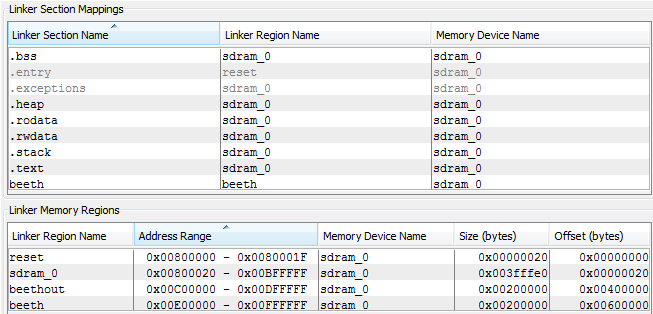
\includegraphics[width = \textwidth]{linkersections.PNG}
	\end{center}
	\caption{The linker sections and memory regions defined in the linker script.}
	\label{fig:linkersections}
\end{figure}

The audio data that will be filtered needs to be copied onto the SDRAM. We found that the smoothest way to achive this is to edit the linker script to reserve a memory region for the data. This is easily done using the Board Support Package Editor, as shown in Figure~\ref{fig:linkersections}.
Two megabytes is reserved for the input data, and another two megabytes for output data.

In order to get the 2MB data file onto the SDRAM, we define a linker section called \verb"beeth". We then generate a relocatable object file using the command line linker tool, and finally rename the automatically named data section to \verb"beeth".
The commands are as follows:

\begin{lstlisting}[frame=, aboveskip=3mm, belowskip=3mm]
nios2-elf-ld -r -b binary -o beeth.o beeth5_noise.bin
nios2-elf-objcopy --rename-section .data=beeth beeth.o beethsect.o
\end{lstlisting}

To link this object file to the rest of the system, we append the following to the end of the user-modifiable section of the Makefile:

\begin{lstlisting}[frame=, aboveskip=3mm, belowskip=3mm]
# User object files
OBJS := beethsect.o
\end{lstlisting}

As this object file is linked with the rest of the system, the following symbols are automatically defined:

\begin{lstlisting}[frame=, aboveskip=3mm, belowskip=3mm]
_binary_beeth5_noise_bin_start
_binary_beeth5_noise_bin_size
_binary_beeth5_noise_bin_end
\end{lstlisting}

This makes for seamless system integration, as these symbols can readily be used in the C code. Furthermore, the data itself will automatically be included in the .elf, and will as such automatically be downloaded to the target without requiring any extra user action.

We found that the easiest way to retrieve data from the system was to use the memory manipulation commands of GDB. That is, to download the memory contents to a file on the host machine, the following command is used in the GDB console:

\begin{lstlisting}[frame=, aboveskip=3mm, belowskip=3mm]
dump binary memory <file> <start_addr> <end_addr>
\end{lstlisting}

% subsection operation (end)

% section notch_filter (end)

\end{document}
